\documentclass{ximera}
\author{Jim Talamo \and Bart Snapp}
\newcommand{\RR}{\mathbb R}
\renewcommand{\d}{\,d}
\newcommand{\dd}[2][]{\frac{d #1}{d #2}}
\renewcommand{\l}{\ell}
\newcommand{\ddx}{\frac{d}{dx}}
\newcommand{\dfn}{\textbf}
\newcommand{\eval}[1]{\bigg[ #1 \bigg]}


\outcome{Define a sequence.}
\outcome{Write the first several terms of a sequence using an explicit formula.}
\outcome{Write the first several terms of a sequence using a recurrence relation.}
\outcome{Find an explicit formula for a sequence given recursively.}
\outcome{Find a recurrence relation for a sequence given explicitly.}
\outcome{Use a given sequence to create new sequences.}

\title[Dig-In:]{Sequences}

\begin{document}
\begin{abstract}
  A sequence is an ordered list of numbers.
\end{abstract}
\maketitle

Let's get to the heart of the matter:

\begin{definition}
  A \dfn{sequence} is an ordered list of numbers.
\end{definition}

In this course, we will generally work with infinite sequences.  Unless otherwise specified, you should assume that the sequences we discuss have infinitely many terms but other books may use other conventions.

For example, here is a sequence:
\[
1,1, 2, 3, 5, 8, 13, 21, \ldots
\]
Here is another sequence:

\[
e, 3\pi, \arctan(27), \frac{1}{42}, \ldots
\]


Note that numbers in the list can repeat.  The dots ``\ldots'' signify that the list keeps going forever.  We often want to refer to a specific term in this list, so we introduce some standard notation.
%want a notation environment
\begin{definition} The notation $\left\{a_n\right\}_{n=1}$ will be used to denote the ordered list of numbers below.

\[
a_1, a_2,  a_3, \ldots
\]
\end{definition}

The subscript in the above notation is called the \emph{index} and describes how we reference the first term.  In many instances, we index sequences starting at $n=0$ or $n=1$ but would like to have the freedom to make other choices should it be convenient.  Thus, there is no unique way to describe a given list of numbers.  For example, the sequence:

\[
1,1, 2, 3, 5, 8, 13, 21, \ldots
\]
could be described by $\left\{a_n\right\}_{n=1}$, where $a_1=1$, $a_2=1$, $a_3=2$, etc or by  $\left\{b_n\right\}_{n=3}$, where $b_3=1$, $b_4=1$, $b_5=2$, etc.

\begin{remark}
Many authors denote sequences using other notation.  Some other common ones you may see are listed below. 

\begin{align*}
  &a_n = f(n), n \geq 1   \\
  & \left\{a_n\right\}_{n=1}^\infty, \\
  & \left(f(n)\right)_{n=1}^\infty \\
\end{align*}
In this text, we will write $\left\{a_n\right\}$ to refer to the sequence and $a_n$ to refer to a specific term in the sequence.

\end{remark}

\begin{question}
  Consider the sequence
  \[
  1, 2, 4, 8, 16, \dots.
  \]
  Which number comes next?
  \begin{multipleChoice}
    \choice{$32$}
    \choice{$31$}
    \choice{$18$}
    \choice[correct]{There is no way to know.}
  \end{multipleChoice}

While there seems to be a pattern, without giving a rule that defines the successive terms, it's impossible to establish what the next one is. 

\end{question}

To explore further, here are two different sequences whose first five terms are the same as the example above.

\begin{example}
  Let $a_n = 2^{n-1}$.  Write down $a_1$, $a_2$, $a_3$, $a_4$, $a_5$, and
  $a_6$.
  \begin{explanation}
    By using the given formula, we find the following.
    \begin{align*}
      a_1 &= \answer[given]{1} & a_2 &= \answer[given]{2} & 
      a_3 &= \answer[given]{4} & 
      a_4 &= \answer[given]{8} & 
      a_5 &= \answer[given]{16} & 
      a_6 &= \answer[given]{32}
    \end{align*}
  \end{explanation}
\end{example}


\begin{example}
  Consider a circle with $n$ points on it. Let $b_n$ be the maximum
  number of regions produced by connecting these points with
  chords. Write down $b_1$, $b_2$, $b_3$, $b_4$, $b_5$, and $b_6$.
  \begin{explanation}
    A good way to approach this problem is to start drawing
    pictures and counting regions.
    \begin{itemize}
      \item \begin{tikzpicture}[framed,scale=1,baseline=-1ex]      
            \tkzDefPoint(0,0){O} 
            \tkzDefPoint(1,0){A} 
            \tkzDrawCircle[color=penColor,very thick](O,A)
            \tkzDrawPoint[color=penColor,fill=penColor](A)
      \end{tikzpicture} We see that $b_1 = \answer[given]{1}$.
      \item \begin{tikzpicture}[framed,scale=1,baseline=-1ex]      
            \tkzDefPoint(0,0){O} 
            \tkzDefPoint(1,0){A} 
            \tkzDefPoint(-1,0){B}
            \tkzDrawCircle[color=penColor,very thick](O,A)
            \tkzDrawPoint[color=penColor,fill=penColor](A)
            \tkzDrawPoint[color=penColor,fill=penColor](B)
            \tkzDrawSegment[color=penColor](A,B)
      \end{tikzpicture} We see that $b_2 = \answer[given]{2}$.
      \item \begin{tikzpicture}[framed,scale=1,baseline=-1ex]      
            \tkzDefPoint(0,0){O} 
            \tkzDefPoint(1,0){A} 
            \tkzDefPoint(-.6,.8){B}
            \tkzDefPoint(-.6,-.8){C}
            \tkzDrawCircle[color=penColor,very thick](O,A)
            \tkzDrawPoint[color=penColor,fill=penColor](A)
            \tkzDrawPoint[color=penColor,fill=penColor](B)
            \tkzDrawPoint[color=penColor,fill=penColor](C)
            \tkzDrawSegment[color=penColor](A,B)
            \tkzDrawSegment[color=penColor](A,C)
            \tkzDrawSegment[color=penColor](B,C)
      \end{tikzpicture} We see that $b_3 = \answer[given]{4}$.
      \item \begin{tikzpicture}[framed,scale=1,baseline=-1ex]      
            \tkzDefPoint(0,0){O} 
            \tkzDefPoint(.6,.8){A} 
            \tkzDefPoint(-.6,.8){B}
            \tkzDefPoint(-.6,-.8){C}
            \tkzDefPoint(.6,-.8){D}
            \tkzDrawCircle[color=penColor,very thick](O,A)
            \tkzDrawPoint[color=penColor,fill=penColor](A)
            \tkzDrawPoint[color=penColor,fill=penColor](B)
            \tkzDrawPoint[color=penColor,fill=penColor](C)
            \tkzDrawPoint[color=penColor,fill=penColor](D)
            \tkzDrawSegment[color=penColor](A,B)
            \tkzDrawSegment[color=penColor](A,C)
            \tkzDrawSegment[color=penColor](A,D)
            \tkzDrawSegment[color=penColor](B,C)
            \tkzDrawSegment[color=penColor](B,D)
            \tkzDrawSegment[color=penColor](C,D)
      \end{tikzpicture} We see that $b_4 = \answer[given]{8}$.
        \item \begin{tikzpicture}[framed,scale=1,baseline=-1ex]      
            \tkzDefPoint(0,0){O} 
            \tkzDefPoint(1,0){A} 
            \tkzDefPoint(.27,.96){B}
            \tkzDefPoint(-.8,.6){C}
            \tkzDefPoint(-.8,-.6){D}
            \tkzDefPoint(.33,-.95){E}
            \tkzDrawCircle[color=penColor,very thick](O,A)
            \tkzDrawPoint[color=penColor,fill=penColor](A)
            \tkzDrawPoint[color=penColor,fill=penColor](B)
            \tkzDrawPoint[color=penColor,fill=penColor](C)
            \tkzDrawPoint[color=penColor,fill=penColor](D)
            \tkzDrawPoint[color=penColor,fill=penColor](E)
            \tkzDrawSegment[color=penColor](A,B)
            \tkzDrawSegment[color=penColor](A,C)
            \tkzDrawSegment[color=penColor](A,D)
            \tkzDrawSegment[color=penColor](A,E)
            \tkzDrawSegment[color=penColor](B,C)
            \tkzDrawSegment[color=penColor](B,D)
            \tkzDrawSegment[color=penColor](B,E)
            \tkzDrawSegment[color=penColor](C,D)
            \tkzDrawSegment[color=penColor](C,E)
            \tkzDrawSegment[color=penColor](D,E)
        \end{tikzpicture} We see that $b_5 = \answer[given]{16}$.
        \item \begin{tikzpicture}[framed,scale=1,baseline=-1ex]      
            \tkzDefPoint(0,0){O} 
            \tkzDefPoint(1,0){A} 
            \tkzDefPoint(0,1){B}
            \tkzDefPoint(-.8,.6){C}
            \tkzDefPoint(-.8,-.6){D}
            \tkzDefPoint(0,-1){E}
            \tkzDefPoint(.7,-.71){F}
            \tkzDrawCircle[color=penColor,very thick](O,A)
            \tkzDrawPoint[color=penColor,fill=penColor](A)
            \tkzDrawPoint[color=penColor,fill=penColor](B)
            \tkzDrawPoint[color=penColor,fill=penColor](C)
            \tkzDrawPoint[color=penColor,fill=penColor](D)
            \tkzDrawPoint[color=penColor,fill=penColor](E)
            \tkzDrawPoint[color=penColor,fill=penColor](F)
            \tkzDrawSegment[color=penColor](A,B)
            \tkzDrawSegment[color=penColor](A,C)
            \tkzDrawSegment[color=penColor](A,D)
            \tkzDrawSegment[color=penColor](A,E)
            \tkzDrawSegment[color=penColor](A,F)
            \tkzDrawSegment[color=penColor](B,C)
            \tkzDrawSegment[color=penColor](B,D)
            \tkzDrawSegment[color=penColor](B,E)
            \tkzDrawSegment[color=penColor](B,F)
            \tkzDrawSegment[color=penColor](C,D)
            \tkzDrawSegment[color=penColor](C,E)
            \tkzDrawSegment[color=penColor](C,F)
            \tkzDrawSegment[color=penColor](D,E)
            \tkzDrawSegment[color=penColor](D,F)
            \tkzDrawSegment[color=penColor](E,F)
            \end{tikzpicture} We see that $b_6 = \answer[given]{31}$.
    \end{itemize}
    While we have made no real argument that these are the maximum
    number of regions, we believe that if the young mathematician draws
    more pictures they will be convinced.
  \end{explanation}
\end{example}


From the two sequences we've just considered, the method of finding
a pattern is \textbf{not enough} when dealing with sequences unless
you understand exactly how the sequence was produced.  However, having
to define each term explicitly is quite cumbersome.  In general, we
want to define a sequence by specifying a rules that will allow us to
write down any term that we want.  There are two important ways that
are generally used to describe a sequence.


\section{Two common methods of representing sequences}

\paragraph{Method One: Explicit Formulas}

\begin{definition}
We say that a sequence $\{a_n\}_{n=1}$ is described by an \dfn{explicit formula} if the term $a_n$ is expressed as a function of $n$.
\end{definition}

Just as real-valued functions were usually expressed by a formula, we
will most often encounter sequences that can be expressed by a
formula.  We say that such sequences are defined \textit{explicitly}, 
or that we have an explicit formula for the sequence.

\begin{example}
Suppose $\{a_n\}_{n=1}$ is a sequence defined by the formula $a_n = 2n+3$.  Write down $a_1$, $a_2$, $a_3$, $a_4$, and $a_5$.

  \begin{explanation}
    By substituting $n=1, 2, 3, 4$ and $5$ into the formula above, we see:
    \begin{align*}
      a_1 &= \answer[given]{5} & 
      a_2 &= \answer[given]{7} & 
      a_3 &= \answer[given]{9} & 
      a_4 &= \answer[given]{11} & 
      a_5 &= \answer[given]{13} 
    \end{align*}
    
Thus, the rule $a_n = 2n+3, n \geq 1$ generates the ordered list below.

\[
5,7,9,11,13, \dots
\]   

There is certainly a pattern that is suggested by the list above. Now that we have an actual rules that gives the terms in the sequence, we can use it to verify that the pattern holds.

  \end{explanation}
  
\end{example}

\begin{warning}
  A common misconception is to confuse the sequence, which is the
  actual ordered list of numbers, with the rule that generates it.
  The sequences $\{a_n\}$ and $\{b_n\}$ given by the rules $a_n =
  (-1)^n$ and $b_n = \cos (\pi \cdot n)$ are different rules which give rise to the \textit{same} sequence (write
  out a few terms to see for yourself).  
  \end{warning}



%\begin{definition}
%  Suppose $\{a_n\}_{n=1}$ and $\{b_n\}_{n=1}$ are sequences.  These
%  sequences are \dfn{equal}\index{sequence!equality} if for all
%  natural numbers $n$, we have $a_n = b_n$.
%
%  More generally, two sequences $\{a_n\}$ and $\{b_n\}$ are
%  \dfn{equal} if, after describing their terms by using the same initial index $n=N$, we have
%  \[
%  a_n = b_n \quad \text{for all $n \geq N$.}
%  \]
%  
%  This is the formal way that we say that these sequences are the same ordered list of numbers.
%\end{definition}


%Put another way, sequences are the same if they have the same set of
%valid indices, and produce the same real numbers for each of those
%indices---regardless of whether the given ``rules'' or procedures for
%computing those sequences resemble each other in any way.

\paragraph{Method Two: Recursive Formulas}

\begin{definition}
We say that a sequence $\{a_n\}_{n=1}$ is described by a \dfn{recursive formula} if the formula for $a_n$ depends on at least one of the previous terms in the sequence.
\end{definition}

We start by defining the first few elements of the sequence, and then describe how later elements are computed in terms of previous elements.

\begin{example}
 Suppose that $\{a_n\}_{n=1}$ is a sequence defined by the formula $a_{n+1} = a_n+2$, where $a_1 = 5$.  Write down $a_2$, $a_3$, $a_4$, and $a_5$.
 
 \begin{explanation}
 Substituting in $n=2$ gives the following.
 
 \[
 a_2 = a_{\answer[given]{1}}+2 = \answer[given]{5}+2 = \answer[given]{7}
 \]
 We can now plug in $n=3$ and use the previous result for $a_2$ to find $a_3$:
  \[
 a_3 = a_{\answer[given]{2}}+2 = \answer[given]{7}+2 = \answer[given]{9}
 \]
 Continuing, we find $a_4 = \answer[given]{11}$ and $a_5 = \answer[given]{13}$.
 
The rule $a_{n+1} = a_n+2, n \geq 1$ thus generates the ordered list:

\[
5,7,9,11,13, \dots
\]   

 \end{explanation}
\end{example}

\begin{remark} Note that both the explicit formula and recursive formula in the previous examples seem to generate the same list of numbers.  While writing out more and more terms suggests this is the case, it is not a sufficient argument to conclude that both rules generate the same sequence.  What we can do is verify whether the explicit formula satisfies the same rule given by the recursive one.  Letting $a_n = 2n+3$, we find:
\begin{align*}
a_{n+1} &= 2\left(\answer[given]{n+1}\right)+3 \\
&= 2n+5 \\
&= \left(2n+3\right) +2 \\
&= a_n+2
\end{align*}  

The term $a_n = 2n+3$ satisfies the requirement $a_{n+1}=a_n+2$, so the different looking formulas $a_n = 2n+3, n \geq 1$ and $a_{n+1}=a_n+2, a_1=5$ actually represent the same sequence.
\end{remark}

%  \begin{remark}
%  The idea of ``recognizing a pattern" and using it to generate more terms for the above example can be made more mathematically explicit through the notion of \emph{mathematical induction}.  The young mathematician may hypothesize that based on the pattern in the recursive formula:
%  
%  \[
%  a_n = a_{n-1}+2, a_1 = 5
%  \]
%  
%  the explicit rule $a_n = 2n+3$ for $n \geq 1$ generates the same sequence, and may prove beyond doubt that this is indeed the case by using induction.  We leave it to the curious young mathematician to research and explore this idea further.
%  \end{remark}
  
  
  
  










\section{Two important types of sequences}

The previous example of a sequence is actually an example of a very common type of sequence called an \emph{arithmetic sequence} .  
%{Mathematically, the word \dfn{family}
%  does not have an entirely precise definition; a family of things is
%  a \dfn{collection} or a \dfn{set} of things, but family
%  also has a connotation of some sort of relatedness.} 

\begin{definition}
  An \dfn{arithmetic sequence} (sometimes called an arithmetic
  progression)\index{arithmetic progression} is a sequence for which the
  difference between subsequent elements is constant.
\end{definition}


\begin{example}
  Here is an example of an arithmetic sequence.
  \begin{image}
  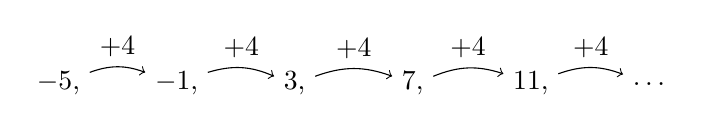
\begin{tikzpicture}[node distance=1.5cm]
    \node (a1) {$-5$,};
    \node (a2) [right of=a1] {$-1$,};
    \node (a3) [right of=a2] {$3$,};
    \node (a4) [right of=a3] {$7$,};
    \node (a5) [right of=a4] {$11$,};
    \node (a6) [right of=a5] {$\ldots$};

    \path[->] (a1) edge [bend left=20] node[above]{$+4$} (a2);
    \path[->] (a2) edge [bend left=20] node[above]{$+4$} (a3);
    \path[->] (a3) edge [bend left=20] node[above]{$+4$} (a4);
    \path[->] (a4) edge [bend left=20] node[above]{$+4$} (a5);
    \path[->] (a5) edge [bend left=20] node[above]{$+4$} (a6);
  \end{tikzpicture}
  \end{image}
  This sequence is given explicitly by the function $a_n=\answer[given]{4n-9}$,
  or recursively by the rule $a_1 = \answer[given]{-5}$ and $a_{n+1} = a_n
  + \answer[given]{4}$. The difference between subsequent elements in this sequence is always four.
\end{example}

In general, an arithmetic sequence in which subsequent terms differ
by $m$ can be written as
\[
a_n = m (n-1) + a_1.
\]
Alternatively, we could describe an arithmetic sequence recursively,
by giving a starting value $a_1$, and using the rule that $a_{n} =
a_{n-1} + m$.  You should check that this general statement holds for our 
two previous examples.


\begin{remark}
The arithmetic mean of two numbers $a$ and $b$ is defined to be $\frac{a+b}{2}$. Note that every term in an arithmetic sequence is the \dfn{arithmetic mean} of its two neighbors.  
\end{remark}


%\subsection{Arithmetic sequences in the wild}
%BADBAD it would be good to have examples...

A second family of sequences we consider are geometric sequences.  

\begin{definition}
  A \dfn{geometric sequence} (sometimes called a geometric
  progression)\index{geometric progression} is a sequence for which the
  ratio between subsequent elements is constant.
\end{definition}

\begin{example}
  Here is an example of a geometric sequence.
  \begin{image}
    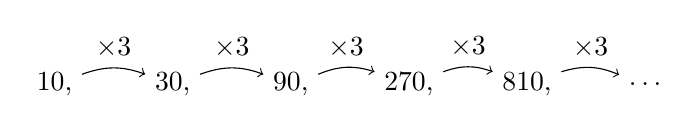
\begin{tikzpicture}[node distance=1.5cm]
    \node (a1) {$10$,};
    \node (a2) [right of=a1] {$30$,};
    \node (a3) [right of=a2] {$90$,};
    \node (a4) [right of=a3] {$270$,};
    \node (a5) [right of=a4] {$810$,};
    \node (a6) [right of=a5] {$\ldots$};

    \path[->] (a1) edge [bend left=20] node[above] {$\times 3$} (a2);
    \path[->] (a2) edge [bend left=20] node[above] {$\times 3$} (a3);
    \path[->] (a3) edge [bend left=20] node[above] {$\times 3$} (a4);
    \path[->] (a4) edge [bend left=20] node[above] {$\times 3$} (a5);
    \path[->] (a5) edge [bend left=20] node[above] {$\times 3$} (a6);
  \end{tikzpicture}
  \end{image}
  This sequence is given explicitly by the function $a_n=\answer[given]{10\cdot
    3^{n-1}}$, or recursively by the rule $a_1 = \answer[given]{10}$ and
  $a_{n+1} = \answer[given]{3}\cdot a_n$. The ratio between any subsequent elements of our sequence is three.
\end{example}

A geometric sequence can also decrease as it progresses.

\begin{example}
  Here is an example of a geometric sequence.
  \begin{image}
    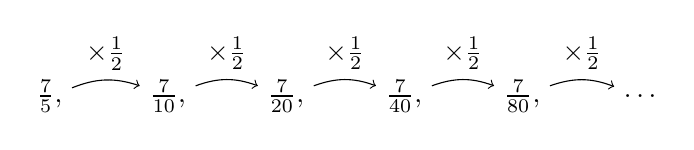
\begin{tikzpicture}[node distance=1.5cm]
    \node (a1) {$\frac{7}{5}$,};
    \node (a2) [right of=a1] {$\frac{7}{10}$,};
    \node (a3) [right of=a2] {$\frac{7}{20}$,};
    \node (a4) [right of=a3] {$\frac{7}{40}$,};
    \node (a5) [right of=a4] {$\frac{7}{80}$,};
    \node (a6) [right of=a5] {$\ldots$};

    \path[->] (a1) edge [bend left=20] node[above] {$\times\frac{1}{2}$} (a2);
    \path[->] (a2) edge [bend left=20] node[above] {$\times\frac{1}{2}$} (a3);
    \path[->] (a3) edge [bend left=20] node[above] {$\times\frac{1}{2}$} (a4);
    \path[->] (a4) edge [bend left=20] node[above] {$\times\frac{1}{2}$} (a5);
    \path[->] (a5) edge [bend left=20] node[above] {$\times\frac{1}{2}$} (a6);
  \end{tikzpicture}
  \end{image}
  This sequence is given by the function $a_n=\answer[given]{\left(\frac{7}{5}\right)\cdot
    \left(\frac{1}{2}\right)^{n-1}}$, or the recursive rule $a_1 = \answer[given]{\frac{7}{5}}$ and
  $a_{n+1} = \answer[given]{\left(\frac{1}{2}\right)}\cdot a_n$. The ratio between subsequent terms 
  of this sequence is always one half.
\end{example}

In general, a geometric sequence $\{a_n\}_{n=0}$ in which the ratio between
subsequent terms is $r$ can be written as
\[
a_n = a_0 \cdot r^{n-1}.
\]
Alternatively, we could describe a geometric sequence
recursively, by giving a starting value $a_0$, and using the rule that
$a_{n} = r \cdot a_{n-1}$.  As usual, you should check that these general 
rules hold for the specific examples we've considered.

\begin{remark}
The
geometric mean of two numbers $a$ and $b$ is defined to be
$\sqrt{ab}$. Note that every term is the \dfn{geometric mean} of its two neighbors.   

%Of course, that raises another question: why is the geometric mean
%called \textit{geometric?}  One geometric interpretation of the
%geometric mean of $a$ and $b$ is this: the geometric mean is the side
%length of a square whose area is equal to that of the rectangle having
%side lengths $a$ and $b$.
\end{remark}
%


\section{Generating new sequences from other sequences}


Once we have defined a given sequence, we make new sequences from it.  Some of the new sequences we can generate allow us to answer important questions about the original sequence.  For now we will look at a few of these important sequences in the context of specific examples. 

\begin{example}
Suppose that $\{a_n\}_{n=1}$ is defined by the explicit formula below.

\[
a_n = 3n-1, n \geq 1
\]

Write out the first six terms in the sequence $\{a_n\}$.
\begin{explanation}
  The first few terms are:
    \begin{align*}
      a_1 &= \answer[given]{2} & 
      a_2 &= \answer[given]{5} & 
      a_3 &= \answer[given]{8} & 
      a_4 &= \answer[given]{11} & 
      a_5 &= \answer[given]{14}  & 
      a_6 &= \answer[given]{17} 
    \end{align*}
\end{explanation}
\end{example}

We can make new sequences from old sequences.

\begin{example}
By noting that none of the terms in the last sequence are $0$, we
define a new sequence $\{b_n\}_{n=1}$ by the rule:
\[
b_n = \frac{a_{n+1}}{a_n}. 
\]
Write out the first five terms in this new sequence.

\begin{explanation}
Starting with $n=1$ we find the next few terms.

\[      b_1 = \frac{a_{\answer{2}}}{a_{\answer{1}}} = \answer[given]{\frac{5}{2}}       \]
      
Continuing in the same way, we find:     
     \begin{align*}
      	b_2 &=  \answer[given]{\frac{8}{5}}  & 
	b_3 &= \answer[given]{\frac{11}{8}}  & 
	b_4 &= \answer[given]{\frac{14}{11}}  & 
	b_5 &=  \answer[given]{\frac{17}{14}}  & 
    \end{align*}
    
\end{explanation}
    
\end{example}

\begin{example}

Since none of the terms in the original sequence $\{a_n\}$ were
negative, we define another new sequence $\{c_n\}_{n=1}$ by the rule
define another new sequence: $\{c_n\}_{n=1}$ by the rule:
\[
c_n = \sqrt[n]{a_n} .
\]
Write out the first five terms in this new sequence.

\begin{explanation}
Starting with $n=1$ we find  $c_1 = \sqrt[1]{a_1} = \answer[given]{2}.$
      
Continuing in the same way, we find     
     \begin{align*}
      	c_2 &=  \answer[given]{5^{1/2}}  & 
	c_3 &= \answer[given]{8^{1/3}}   & 
	c_4 &= \answer[given]{11^{1/4}}   & 
	c_5 &=  \answer[given]{14^{1/5}}   
    \end{align*}
    
\end{explanation}
\end{example}

\begin{example}
Define another new sequence $\{s_n\}_{n=1}$ by 

\[
s_n = \sum_{k=1}^n a_k .
\]
Write out the first five terms in this new sequence.

Recall that the notation $\sum_{k=1}^n a_k$ is shorthand notation used to represent the sum $a_1+a_2+\ldots +a_n$.



\begin{explanation}
Starting with $n=1$ we find

\[      s_1 = a_1 = \answer[given]{2}.      \]
      
Continuing in the same way, we find the next few terms.    
     \begin{align*}
      	s_2 &=  a_1 +a_2 = \answer[given]{7}  \\ 
	s_3 &=  a_1 +a_2 + a_3 = \answer[given]{15}   \\ 
	s_4 &=  a_1 +a_2 +a_3 +a_4= \answer[given]{26}  \\ 
	s_5 &=  a_1 +a_2 +a_3+a_4+a_5= \answer[given]{40}    
    \end{align*}
Note that there are two ways to compute each of the terms above.  One way is to perform the explicit addition each time, but the clever reader may notice that there is a faster way.  For instance, if we have already computed $s_3$, there is a way to use it to find $s_4$ quickly.

\begin{image}
  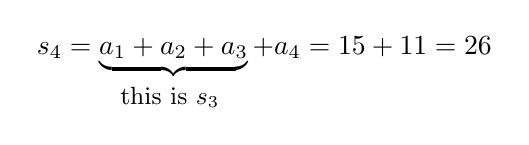
\begin{tikzpicture}
        \node at (0,0) {
          $s_4 = \underbrace{a_1+a_2+a_3} + a_4 = 15+11 =26$
        };
        \node at (-1.2,-.5) {\small{this is $s_3$}};
      \end{tikzpicture}
  \end{image}

Of course, there is a more general observation.

\begin{image}
  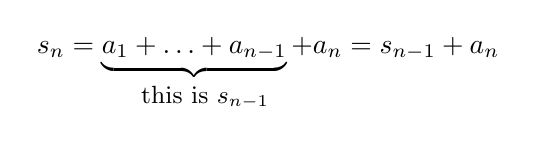
\begin{tikzpicture}
        \node at (0,0) {
          $s_n = \underbrace{a_1+\ldots+a_{n-1}} + a_n = s_{n-1} + a_n$
        };
        \node at (-.8,-.5) {\small{this is $s_{n-1}$}};
      \end{tikzpicture}
  \end{image}
so that in this example, where $a_n = 3n-1$, we have a recursive formula for $\{s_n\}_{n=1}$.

\[
s_n = s_{n-1} + (3n-1), \qquad s_1 =2
\]  
It can be shown that the recursive rule $s_n = s_{n-1} + (3n-1), s_1
=2$ and the explicit formula $s_n = \frac{3n^2+n}{2} , n \geq 1$
represent the same sequence.  We leave this to the curious reader as
an exercise.    
\end{explanation}
\end{example}


%\begin{remark}
%  To do this, we must verify first that the sequences start at the same value.  Indeed, by setting $n=1$ into the explicit formula, we find $s_1 = \answer[given]{2}$.  To proceed, we can show that the sequence given by the explicit formula also satisfies the recursive one.  We do this by taking the explicit formula and substituting it into the recursive one.  
%
%For $n \geq 2$, by setting $s_n = \frac{3n^2+n}{2}$, we find $s_{n-1} = \frac{3\left(\answer{n-1}\right)^2+\left(\answer{n-1}\right)}{2}$, and after a little algebra: $s_{n-1} = \frac{3n^2-5n+2}{2}$.  Thus, we can check whether this satisfies $s_n = s_{n-1} + (3n-1)$:
%
%\begin{align*}
% s_{n-1} + (3n-1) &= \frac{3n^2-5n+2}{2} +3n-1 \\
% &=  \frac{3n^2-5n+2}{2} +(3n-1) \cdot \frac{2}{2} \\ 
% &= \frac{3n^2-5n+2}{2} + \frac{6n-2}{2} \\
% &= \frac{3n^2+n}{2} 
%\end{align*}
%
%This is precisely the expression for $s_n$.
%
%Note that establishing that the sequences start at the same value is important here.  The general philosophy here was to show that the first term in each sequence is the same, and the above computations verify that for \emph{any} term with $n \geq 2$, both rules generate the same result.  Had we specified a different starting value for the recursive formula, the rule $s_n = \frac{3n^2+n}{2}$ would still satisfy the recursive relationship $s_n = s_{n-1} + (3n-1)$, but each expression would generate a different list of numbers.
%
%\end{remark}
%
%\begin{remark}
%The sequences in the previous example will all play an important role in the development that follows.  We will see how they arise in the context of answering a fundamental question introduced in the next section, but it is worth mentioning them now as new sequences that can be constructed from a given sequence.
%\end{remark}
%
%%Here is an example with a real-world context:
%%
%%\begin{example}
%%  Suppose that when a ``super-ball'' is dropped from some height, it
%%  bounces to $90\%$ of the original height. Let $b_1$ be the height
%%  the ball bounces after it is dropped from a height of $3$
%%  meters. Let $b_2$ be the height the ball bounces next, and so on.
%%  Find formulas, both explicit and recursive, for $b_n$.
%%  \begin{explanation}
%%    The first bounce has a height of
%%    \[
%%    b_1 = 0.9\cdot 3
%%    \]
%%    and the second bounce has a height of 
%%    \[
%%    b_2 = 0.9(0.9\cdot 3) = 0.9^2 \cdot 3.
%%    \]
%%     To compute the height of each bounce, one simply multiplies the
%%    previous height by $0.9$, and hence this is a geometric sequence with
%%    explicit formula $b_n = \answer[given]{0.9^n\cdot 3}$ and recursive formula $b_1 =
%%    \answer[given]{0.9\cdot 3}$ and $b_n = \answer[given]{0.9}\cdot b_{n-1}$.
%%  \end{explanation}
%%\end{example}
%%
%%
%%Here is an example that is at the foundations of our number system:
%%
%%\begin{example}
%%  Consider the number
%%  \[
%%  \frac{1}{3} = 0.3333333333\dots.
%%  \]
%%  Let's think of this number in stages.  Let $p_1$ be the value of the digit to the right of the decimal
%%  point.  In other words, let $p_1$ be the number you would get if you left the first digit alone, and changed every other digit to a zero. Let $p_2$ be the value of the second digit to the right, and so
%%  on. Find formulas, both explicit and recursive, for $p_n$.
%%  \begin{explanation}
%%    The first digit to the right of the decimal point is $3$ and its
%%    value is $p_1 = 0.3$. The next digit has a value of $p_2 =
%%    0.03$. The next digit has a value of $p_3 = 0.003$. To find the
%%    value of each digit, we multiply the previous digit by
%%    $\frac{1}{10}$. Hence this is a geometric sequence with explicit
%%    formula $p_n = \answer[given]{\left(\frac{1}{10}\right)^n\cdot 3}$ and recursive
%%    formula $p_1 =\answer[given]{0.3}$ and $p_n = \answer[given]{\left(\frac{1}{10}\right)}\cdot
%%    p_{n-1}$.
%%  \end{explanation}
%%\end{example}
%
%
%%MOVED TO EXERCISES.%%%
%
%%\section{Unsolved mysteries}
%%
%%To whet the appetite of the curious young mathematician further, we discuss an open problem in mathematics.
%%
%%\subsection{Collatz sequences}
%%
%%A particularly interesting example of a recursive sequence with which to amuse your friends---or distract
%%your enemies is as follows:
%%
%%\begin{example}
%%  Let's start our sequence with $a_1 = 6$.  Subsequent terms are
%%  defined using the rule
%%  \[
%%  a_n =
%%  \begin{cases}
%%    a_{n-1} / 2 &\text{if $a_{n-1}$ is even,} \\
%%    3a_{n-1} + 1 &\text{if $a_{n-1}$ is odd.}
%%  \end{cases}
%%  \]
%%  Let's compute $a_2$.  Since $a_1$ is even, we follow the
%%  instructions in the first line, to find that $a_2 = a_1/2 =
%%  \answer[given]{3}$. To compute $a_3$, note that $a_2$ is odd so we
%%  follow the instruction in the second line, and $a_3 = 3 a_2 + 1 = 3
%%  \cdot 3 + 1 = \answer[given]{10}$.  Since $a_3$ is even, the first
%%  line applies, and $a_4 = a_3 / 2 = 10 / 2 = \answer[given]{5}$.  But
%%  $a_4$ is odd, so the second line applies, and we find $a_5 = 3 \cdot
%%  5 + 1 = \answer[given]{16}$.  And $a_5$ is even, so $a_6 = 16 / 2 =
%%  \answer[given]{8}$.  And $a_6$ is even, so $a_7 = 8/4 = 4$.  And
%%  $a_7$ is even, so $a_8 = 4 / 2 = \answer[given]{2}$, and then $a_9 =
%%  2/2 = \answer[given]{1}$.  Oh, but $a_9$ is odd, so $a_{10} = 3
%%  \cdot 1 + 1 = \answer[given]{4}$.  And it repeats.  Let's write down
%%  the start of this sequence:
%%  \[
%%  6,\, %1 
%%  3,\, %2
%%  10,\,  %3
%%  5,\,  %4
%%  16,\,  %5
%%  8,\,  %6
%%  4,\,  %7
%%  2,\,  %8
%%  1,\,  %9
%%  4,\, %10
%%  2,\, %11
%%  1,\, %12
%%  \overbrace{4,\, %10
%%    2,\, %11
%%    1,}^{\text{repeats}}\, %12
%%  4,\, %10
%%  \ldots
%%  \]
%%  What if we had started with a number other than six?  What if we set
%%  $a_1 = 25$ but then we used the same rule?  In that case, since
%%  $a_1$ is odd, we compute $a_2$ by finding $3 a_1 + 1 = 3 \cdot 25 +
%%  1 = 76$.  Since $76$ is even, the next term is half that, meaning
%%  $a_3 = 38$.  If we keep this up, we find that our sequence begins
%%  \begin{align*}
%%    &25,\, 76,\, 38,\, 19,\, 58,\, 29,\, 88,\, 44,\, 22,\, 11,\, 34,\, 17,\, 52,\, 26, \\
%%    &13,\, 40,\, 20,\, 10,\, 5,\, 16,\, 8,\, 4,\, 2, \, 1, \, \ldots
%%  \end{align*}
%%  and then it repeats ``4, 2, 1, 4, 2, 1, \ldots'' just like before.
%%  Does this always happen?  Is it true that no matter which positive
%%  integer you start with, if you apply the half-if-even, $3x+1$-if-odd
%%  rule, you end up getting stuck in the ``4, 2, 1, \ldots'' loop?
%%  That this is true is the \dfn{Collatz conjecture}; it has been
%%  verified for all starting values below $5 \times 2^{60}$.  Nobody
%%  has found a value which doesn't return to one, but for all anybody
%%  knows there \textit{might} well be a very large initial value which
%%  doesn't return to one; nobody knows either way.  It is an unsolved
%%  problem in mathematics.
%%\end{example}
%
%
%%\subsection{Perfect numbers}
%%
%%The notion of a perfect number is over two thousand years old.
%%
%%\begin{definition}
%%  A whole number $P$ is a \dfn{perfect number} if the sum of the
%%  positive divisors less than $P$ is equal to $P$.
%%\end{definition}
%%The number $6$ is perfect, since the positive divisors less than $6$
%%are $1$, $2$, and $3$; and $1+2+3 = 6$.  Here we list the first nine
%%perfect numbers:
%%\begin{align*}
%%P_1 &= 6\\
%%P_2 &= 28\\
%%P_3 &= 496\\
%%P_4 &= 8128\\
%%P_5 &= 33550336\\
%%P_6 &= 8589869056\\
%%P_7 &= 137438691328\\
%%P_8 &= 2305843008139952128\\
%%P_9 &= 2658455991569831744654692615953842176
%%\end{align*}
%%For a complete list, see
%%\url{http://en.wikipedia.org/wiki/List_of_perfect_numbers}.  Note,
%%every number in the list above is even, hence we are lead to a question:
%%
%%
%%\begin{question}
%%  Are there any odd perfect numbers?
%%  \begin{prompt}
%%    \begin{multipleChoice}
%%      \choice{yes}
%%      \choice{no}
%%      \choice[correct]{nobody knows}
%%    \end{multipleChoice}
%%  \end{prompt}
%%\end{question}
%%
%%Nobody knows the answer to this question. In 2012, Ochem and Rao
%%published the result that there are no odd perfect numbers less than
%%$10^{1500}$. This is an \textbf{enormous} number, and it cannot be put
%%in perspective. Consider this: It is estimated that the mass of the
%%\textbf{universe} is less than $10^{61}$ kilograms, and $10^{1500}$ is
%%unfathomably larger.
%
%%ADD THOUGHTS

\begin{quote}
``Obvious" is the most dangerous word in mathematics" -E.T. Bell
\end{quote}

\end{document}
